%%
%% Anthony Mallet - Sun Dec  8 2002-2009
%% Copyright (C) 2002-2009 LAAS/CNRS 
%%
\documentclass[a4paper,landscape,smooth]{show}
\usepackage{depend,aeguill,cartouche}
\usepackage[dpi=100,resample]{docfig}
\usepackage[T1]{fontenc}
\usepackage[latin1]{inputenc}

\context{\vfill}
\title{Introducing Tk}
\author{Anthony Mallet\\ based on E.J. Friedman-Hill's slides}
\date{November 2009}

\newcommand{\tclex}[2]{\texttt{#1}\\$\rightarrow$ \texttt{#2}}

\begin{document}
\maketitle

% =======================================================================

\begin{part}{Introduction}{The Tk toolkit}
   \vfill
   \begin{bitemize}{color@bulle}
      \item {\bf problem}: building an application with a GUI is hard.
        Even more if portability is wanted. 

      \item {\bf Bad solutions} : 
	 C++, object oritented toolkits, Java AWT, ...
         Little benefits: still programming a quite low level.

      \item {\bf Good solution}: 
        Raise the programming level. Use a scripting langage (Tcl) to
        create and manage interfaces.
   \end{bitemize}
   \vfill
   (Arguments by {\bf E.J. Friedman-Hill})
   \vfill
\end{part}

% -----------------------------------------------------------------------

\begin{tslide}{Example}
   \vfill
   {\tt
   listbox .list -yscroll ".scroll set"\\
   pack .list -side left\\
\\
   scrollbar .scroll -command ".list yview"\\
   pack .scroll -side right -fill y\\
\\
   wm title . "File Browser"\\
   foreach i [lsort [glob * .*]] \{\\
\hspace*{1cm}.list insert end \$i\\ \}\\
   }
   \vfill
   \vbox to0pt{\vss\hfill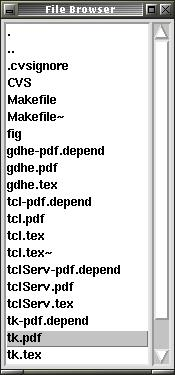
\includegraphics[width=0.3\linewidth]{fig/file-browser.jpg}}
\end{tslide}

% -----------------------------------------------------------------------

\begin{tslide}{Elements of a Tk interface}
   \vfill
   \begin{bitemize}{color@bulle}
      \item new Tcl commands:
	 \begin{itemize}
	    \item create widgets in a hierarchical way.
            \item layout widgets.
            \item bind events to Tcl scripts.
            \item interact with selection, input focus, window managers etc. 
	 \end{itemize}

      \item Set of C libraries :
	 \begin{itemize}
	    \item create new widgets 
	    \item create new geometry managers
	 \end{itemize}
   \end{bitemize}
   \vfill
\end{tslide}

% -----------------------------------------------------------------------

\begin{tslide}{Basic class: {\em widgets}}
   \vfill
   {\bf Widgets}
   \begin{bitemize}{color@bulle}
      \item Windowed gadgets
      \item gadget (n.)\\
	 1. a small mechanical device or appliance.\\
	 2. any object that is interesting for its ingenuity or novelty
	    rather than for its practical use.\\

	 [ perhaps from French ``gachette'': lock catch, trigger,
	    diminutive of gache staple ].
   \end{bitemize}
   \vfill
\end{tslide}

% =======================================================================

\begin{part}{Tk}{Widgets}
   \vfill\small
   \begin{bitemize}{color@bulle}
      \item Toplevel
      \item Frame
      \item Menu, Menubutton
      \item Label, Message
      \item Button, Checkbutton, Radiobutton
      \item Entry, Text
      \item Listbox
      \item Scale, Scrollbar
      \item Canvas
   \end{bitemize}
   \vfill
\end{part}

% -----------------------------------------------------------------------

%\begin{tslide}{Widgets hierarchy}
%   \vfill\begin{center}
%      \docfig[width=0.9\linewidth,psfrag]{tk-hierarchy.fig}
%   \end{center}\vfill
%\end{tslide}

% -----------------------------------------------------------------------

\begin{tslide}{Creating widgets}
   \vfill
   \begin{bitemize}{color@bulle}
      \item Each widget belongs to a class: button, listbox, scrollbar,
	    etc. 
      \item One creation command for each class, used to create instances:\\
	    {\tt button .a.b -text Quit -command exit}\\
	    {\tt scrollbar .x -orient horizontal}
   \end{bitemize}
   \vfill
\end{tslide}

% -----------------------------------------------------------------------

\begin{tslide}{Configuration}
   \vfill
   Configuration options defined by the class. Example for the Button class:\\
   {\tt
      -activebackground -disabledforeground -justify -underline \\
      -activeforeground -font -padx -width \\
      -anchor -foreground -pady -wraplength \\
      -background -height -relief \\
      -bitmap -highlightbackground -state \\
      -borderwidth -highlightcolor -takefocus \\
      -command -highlightthickness -text \\
      -cursor -image -textvariable \\
}

   \vfill
   If options are not explicitely specifed, they can come from Unix X defaults.
   or from Tk defaults.
   \vfill
\end{tslide}

% -----------------------------------------------------------------------

\begin{tslide}{Associating commands to widgets}
   \vfill
   A Tcl command, named after the widget allows to (re)configure 
   and manipulate it:

   {\tt
      button .a.b\\
      .a.b configure -relief sunken\\
      .a.b flash\\
\\
      scrollbar .x\\
      .x set 0.2 0.7\\
      .x get\\

      .a.b configure -foreground\\
      $\rightarrow$ -foreground foreground Foreground blue blue}

    The command is removed from the interpreter when the widget is destroyed.
   \vfill
\end{tslide}

% -----------------------------------------------------------------------

\begin{tslide}{Placement}
   \vfill
   {\bf Geometry management}
   \begin{bitemize}{color@bulle}
      \item {\tt place}
        Absolute positionning of the widget relativelty to its parent.

      \item {\tt pack}
        Positions widgests depending on the size of the parent and of 
        other widgets at the same level.

      \item {\tt grid}
        Puts widgets in a 2-dimensional array.
      \item {\tt frame}
        To create more complex setups.
   \end{bitemize}
   \vfill
\end{tslide}

% -----------------------------------------------------------------------

\begin{tslide}{Connection to Tcl}
   \vfill
   \begin{bitemize}{color@bulle}
      \item Tcl Scripts to let a widget talk to the application 
        or to other widgets 

	    {\tt button .a.b -command exit}\\
	    {\tt scrollbar .s -command ".text yview"}

      \item The application uses the widgets commands to communicate
        with the interface.
   \end{bitemize}
   \vfill
\end{tslide}

% -----------------------------------------------------------------------

\begin{tslide}{Events}
   \vfill
   \begin{bitemize}{color@bulle}
      \item Bind Tcl scripts to user events:
         {\tt bind .b <Control-h> \{puts "control-h"\}}

      \item Naming of events: 

	 {\tt <Double-Control-ButtonPress-1> \\
	       <KeyPress> \\
	       a}

      \item Substitutions : 

	 {\tt bind .c <B1-Motion> \{move \%x \%y\}\\
	       bind .t <KeyPress> \{insert \%A\}}
   \end{bitemize}
   \vfill
\end{tslide}


% -----------------------------------------------------------------------

\begin{tslide}{Other commands}
   \vfill
   \begin{bitemize}{color@bulle}
      \item X11 Selection: 

	 {\tt selection get}

      \item Sending commands to other Tk applications: 

	 {\tt send tgdb "break tkEval.c:200" }

      \item Information on windows:

	 {\tt winfo width .x\\
	       winfo children .\\
	       winfo containing \$x \$y}
   \end{bitemize}
   \vfill
\end{tslide}

% -----------------------------------------------------------------------

\vfill\eject\null\vfill\eject

\end{document}
